% UPAR 2027 Track 1 paper, WACV 2026 author kit (the format required by the RWS workshop at WACV 2027).
\documentclass[10pt,twocolumn,letterpaper]{article}

%%%%%%%%% PAPER TYPE: \usepackage[review,algorithms]{wacv} for the anonymous review version
\usepackage{wacv}

%
% --- inline annotations
%
\newcommand{\red}[1]{{\color{red}#1}}
\newcommand{\todo}[1]{{\color{red}#1}}
\newcommand{\TODO}[1]{\textbf{\color{red}[TODO: #1]}}
% --- disable by uncommenting  
% \renewcommand{\TODO}[1]{}
% \renewcommand{\todo}[1]{#1}


\usepackage{booktabs}
\usepackage{multirow}
\usepackage{amsmath}
\usepackage{graphicx}
\graphicspath{{figs/}}

\definecolor{wacvblue}{rgb}{0.21,0.49,0.74}
\usepackage[pagebackref,breaklinks,colorlinks,allcolors=wacvblue]{hyperref}
\usepackage[capitalize]{cleveref}

\def\wacvPaperID{*****}
\def\confName{WACV}
\def\confYear{2027}
\newcommand{\pts}{\,pts}

\title{Complementary Foundation Encoders and Prior-Corrected Thresholds\\for Cross-Domain Pedestrian Attribute Recognition}

\author{Anonymous Authors\\
UPAR Challenge 2027, Track 1}

\begin{document}
\maketitle

%=====================================================================
\begin{abstract}
A pedestrian attribute recognizer is usually trained on data from some cameras and then used on others. The cameras differ in domain. Resolution, viewpoint and lighting change, and each dataset also labels attributes by its own conventions. Foundation models are pretrained on very large and varied image collections, so their features depend little on any single domain. When they are fine-tuned on a few surveillance datasets, however, they tend to absorb the properties and conventions of those datasets and lose part of this generality. We propose a system that keeps this generality and corrects how decisions are made. First, we combine two foundation models pretrained in different ways, DINOv3 from images alone and CLIP from images with captions. Each is fine-tuned only in its top layers, and their outputs are averaged. Because their pretraining differs, they make different mistakes on a new domain, and their average is more accurate than either. Second, we correct the decision threshold. A threshold of 0.5 is optimal for accuracy on the training data, whereas the challenge metric weighs people with and without an attribute equally, and attribute frequencies differ in the new domain. As a result, rare attributes are under-predicted. We shift the threshold of each attribute according to its frequency, with one coefficient shared by all 40 attributes. The shift is derived from the metric and needs no labels from the new domain. On a dataset held out to simulate a new domain, the two components together add 1.8 points over the best single model. Our system scores 0.7997 Challenge\_Avg on the hidden test set of UPAR 2027 Track~1.
\end{abstract}

\begin{figure*}[t]
\centering
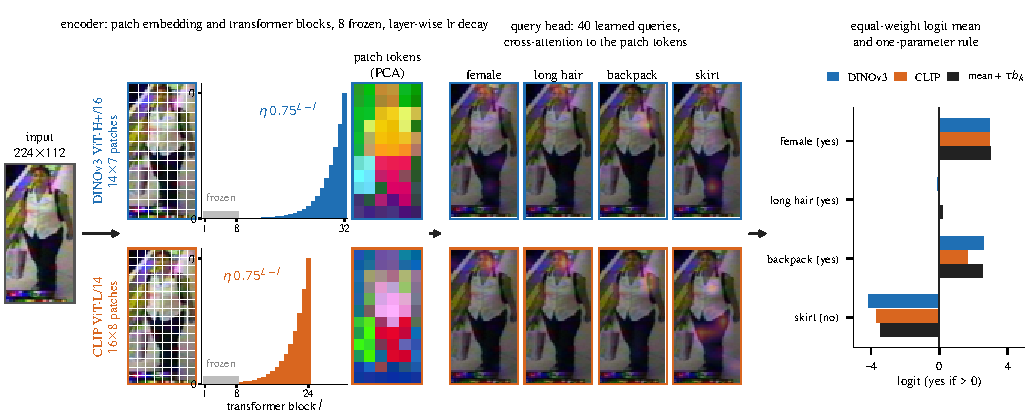
\includegraphics[width=\linewidth]{architecture.pdf}
\caption{Overview of the method on a PETA image. Each row is one encoder: its patch grid, the learning rate of each transformer block during fine-tuning, and its patch tokens shown by their first three principal components. Each attribute query attends to the tokens, and the logits of the two encoders are averaged and shifted by the prior correction. Tokens, attention and logits come from ViT-L members that never saw PETA during training.}
\label{fig:arch}
\end{figure*}

%=====================================================================
\section{Introduction}
\label{sec:intro}

Pedestrian attribute recognition (PAR) predicts properties such as gender, clothing color and carried objects from a crop of a person. It supports searches like ``a woman in a pink top with a backpack'' in surveillance video. In practice the recognizer runs on cameras that were not part of its training data. Standard benchmarks~\cite{peta,pa100k,market} do not test this case, because their training and test images come from the same cameras. The UPAR challenges~\cite{upar,upar23,upar24} do. They train on several public datasets and test on a domain that contributes no training image.

When we simulate this setting by holding out one training dataset, we see two separate problems. First, ranking gets worse. The mean AUC of a strong encoder drops by about four points on the held-out dataset, so positives and negatives are separated less well. Second, the threshold no longer fits. The challenge uses a fixed threshold of 0.5, and the attribute frequencies of a new domain differ from those of the training data. Thresholds fitted on the held-out labels would add about three points, which shows how much the fixed threshold costs.

We propose one component for each problem (\cref{fig:arch}). To improve ranking, we combine two encoders whose pretraining differs. DINOv3~\cite{dinov3} learns from images alone, and CLIP~\cite{clip} learns from images paired with text. Their errors on a new domain differ, so averaging them helps. We fine-tune both only in their upper blocks, which keeps most of their pretrained features. To fix the threshold, we add a correction to each logit that depends on how frequent the attribute is in training. The correction follows from the balanced-accuracy part of the metric, whose optimum does not depend on the attribute frequencies of the new domain. It has one free coefficient for all 40 attributes.

Our contributions are:
\begin{itemize}
\item A two-encoder system for cross-domain PAR. It pairs a self-supervised and an image-text foundation encoder, each with a query head, and averages their logits (\cref{sec:encoders,sec:ensemble}).
\item A prior-corrected threshold with a single coefficient, derived from the challenge metric. It needs no target labels and transfers better than per-attribute thresholds fitted on the training data (\cref{sec:rule,sec:exp_rule}).
\item A study of the design choices that matter on unseen cameras. It shows how to choose the partner encoder, how to combine the encoders and how far to fine-tune them (\cref{sec:exp_partner,sec:exp_design,sec:exp_depth}).
\end{itemize}
The system scores 0.7997 Challenge\_Avg on the hidden test set of UPAR 2027 Track~1.

%=====================================================================
\section{Related Work}
\label{sec:related}

\paragraph{Pedestrian attribute recognition.} DeepMAR~\cite{deepmar} treated PAR as multi-label classification and weighted the loss by attribute frequency. Later methods added modules that localize attributes or model their relations. Jia~\etal~\cite{rethinkpar} showed that many of these gains vanish under a stricter evaluation split. Query-based heads~\cite{q2l,mldecoder} give each label a learned query over the image tokens, and we use such a head. UPAR~\cite{upar} unified four datasets into a common set of 40 attributes, which enables cross-domain evaluation.

\paragraph{Pretrained encoders under domain shift.} With a strong backbone, plain training matches specialized domain generalization methods~\cite{domainbed}. Full fine-tuning can distort pretrained features and lower accuracy under distribution shift~\cite{lpft}, which motivates partial fine-tuning and interpolation with the pretrained weights~\cite{wiseft}. Averaging the weights of several fine-tuned models also improves robustness~\cite{soups,diwa}.

\paragraph{Ensembles.} An ensemble improves when its members are accurate and when they make different errors~\cite{krogh}. Deep ensembles are among the most reliable models under dataset shift~\cite{deepens,ovadia}. We study which of these factors matters when the members are foundation encoders and the metric uses a fixed threshold.

\paragraph{Prior correction.} When class frequencies change, predicted probabilities can be corrected with the ratio of the frequencies~\cite{saerens,lipton}. Adding a scaled log prior to the logits optimizes the balanced error~\cite{logitadj}. Our threshold correction builds on this idea and also removes the shift caused by the DeepMAR loss weights.

%=====================================================================
\section{Method}
\label{sec:method}

\subsection{Task and metric}
\label{sec:task}

Each crop has 40 binary attributes. They cover age (three classes), gender, hair length (three classes), sleeve length, the length and type of the lower garment, twelve upper-body and twelve lower-body colors, and five accessories. The challenge score Challenge\_Avg (Avg) is the harmonic mean of two terms. The first is mA, the balanced accuracy averaged over attributes. The second is instance F1, the F1 score of each image's predicted attribute set, averaged over images. Both terms threshold the predicted probabilities at 0.5.

\subsection{Complementary encoders}
\label{sec:encoders}

A single encoder makes systematic errors on a new domain. Two encoders help only if their errors differ, and errors differ most when the encoders were pretrained differently. We therefore pair DINOv3 ViT-H+/16~\cite{dinov3}, trained by self-distillation on images, with CLIP ViT-L/14~\cite{clip}, trained to match images with captions. Both read a $224\times112$ crop, which gives $14\times7$ patch tokens for DINOv3 and $16\times8$ for CLIP.

Fine-tuning on the three training datasets should change the pretrained features as little as needed. We freeze the patch embedding and the first eight transformer blocks. The other blocks use layer-wise learning-rate decay~\cite{beit}, so block $l$ of $L$ receives the learning rate $\eta\cdot0.75^{L-l}$. \Cref{fig:arch} plots these rates. Most of the update happens in the last few blocks.

\paragraph{Query head.} Each attribute depends on its own region, such as the face for glasses or the legs for a skirt. We use a query head~\cite{q2l,mldecoder}, which gives every attribute a learned query vector. The query attends to the patch tokens with one cross-attention layer of eight heads, and a small MLP and a classifier of that attribute produce its logit. \Cref{fig:arch} shows that the queries focus on the regions of their attributes, even on a dataset the encoders never saw.

\paragraph{Training loss.} We use binary cross-entropy with label smoothing of 0.05 and the DeepMAR weights~\cite{deepmar} $w_k^{+}=e^{1-\pi_k}$ for positives and $w_k^{-}=e^{\pi_k}$ for negatives. Here $\pi_k$ is the frequency of attribute $k$ in the training labels. The weights make rare attributes count more. They also shift the decision of the model, which the threshold correction of \cref{sec:rule} takes into account. Datasets are sampled in proportion to the square root of their size, so that the largest one does not dominate. \Cref{app:config} lists all settings.

\subsection{Logit averaging}
\label{sec:ensemble}

The two encoders give one logit per attribute, $z_k^{\text{DINO}}$ and $z_k^{\text{CLIP}}$. We use their mean $\bar z_k=\frac12(z_k^{\text{DINO}}+z_k^{\text{CLIP}})$. Averaging logits instead of probabilities lets a confident encoder outweigh an uncertain one. We keep the weights equal, because the best weight depends on the target domain, which is unknown. \Cref{sec:exp_design} shows that equal weights are close to the best weight on two held-out domains.

\subsection{Prior-corrected thresholds}
\label{sec:rule}

A threshold of 0.5 is rarely optimal for an attribute that appears in only 2\% of the images. The common fix fits one threshold per attribute on validation data. On a new domain this fails, because those thresholds also learn how the training datasets were labelled (\cref{sec:exp_rule}). We want a correction that needs no target labels and has few parameters.

The mA term of the metric gives such a correction. Balanced accuracy counts errors on positives and negatives equally. Its best decision is therefore the one made as if both classes were equally frequent, whatever the frequencies of the target domain are. For a model calibrated to the training frequency $\pi_k$, this decision is reached by adding $\log\frac{1-\pi_k}{\pi_k}$ to the logit~\cite{saerens,logitadj}. The DeepMAR weights have already shifted the decision by $\log(w_k^{+}/w_k^{-})=1-2\pi_k$. We add only the remaining part:
\begin{equation}
z_k=\bar z_k+\tau\,b_k,\qquad b_k=\log\frac{1-\pi_k}{\pi_k}-(1-2\pi_k).
\label{eq:rule}
\end{equation}
The term $b_k$ is large and positive for rare attributes, so they are predicted more often. For a pink top it is about 2.7. It is negative for frequent attributes, such as trousers. The instance F1 term prefers fewer positive predictions, which works against the mA term. The coefficient $\tau\in[0,1]$ balances the two. At $\tau=0$ the model keeps the decision of the weighted loss, and at $\tau=1$ it takes the decision that is best for mA. We use $\tau=0.42$, set in earlier experiments with single models. The priors $\pi_k$ come from all training and validation labels.

%=====================================================================
\section{Experiments}
\label{sec:experiments}

\subsection{Setup}
\label{sec:setup}

\paragraph{Data.} We train on the UPAR annotations of PA100k, Market1501 and PETA (\cref{tab:data}). The hidden test set has 29{,}248 images from another domain.

\begin{table}[t]
\centering\small
\setlength{\tabcolsep}{3pt}
\resizebox{\columnwidth}{!}{%
\begin{tabular}{@{}lrrl@{}}
\toprule
Dataset & Train & Val & Images \\
\midrule
PA100k~\cite{pa100k} & 79{,}001 & 9{,}986 & outdoor, about 600 cameras \\
Market1501~\cite{market,marketattr} & 10{,}000 & 16{,}458 & one campus, $128\times64$ crops \\
PETA~\cite{peta} & 8{,}668 & 6{,}963 & ten pooled sources \\
\bottomrule
\end{tabular}}
\caption{Training data of UPAR 2027 Track~1.}
\label{tab:data}
\end{table}

\paragraph{Held-out protocol.} We cannot evaluate on the test domain, so we hold out one training dataset instead. Models are trained on two datasets and scored on the validation images of the third. PETA is the main held-out dataset, and Market1501 is a second one. We also report a source score, which is measured on the validation images of the two training datasets. Protocol models train for three epochs. The submitted models train for three epochs on the training and validation images of all three datasets. We report Avg and AUC $\times100$, and differences in points (pts).

\paragraph{Noise.} Four runs of CLIP ViT-L/14 with the same settings score between 81.13 and 81.58 on held-out PETA, and between 82.17 and 82.42 when paired with DINOv3. Differences below about 0.3\pts{} between single runs are therefore not reliable.

\subsection{Contribution of each component}
\label{sec:exp_main}

\Cref{tab:main} builds the system step by step. The prior correction helps every model on both held-out datasets, by 0.6 to 1.2\pts. The pair is better than either encoder on PETA, both before and after the correction. With the correction, it gains 0.8\pts{} over the best single encoder. The two components therefore improve different parts of the error, and their gains add up. On Market1501 the pair is roughly equal to DINOv3 alone, because CLIP is much weaker there. The pair still has the highest AUC on both datasets, which shows that it ranks images better and does not only shift thresholds.

The last row uses thresholds fitted on the held-out labels themselves. This oracle cannot be used in practice, but it shows how much a perfect threshold rule could still add. The remaining gap is 1.85\pts{} on PETA and 1.70\pts{} on Market1501. In earlier experiments we traced most of it to clothing colors, which the datasets label differently. PETA, for example, gives two colors to 12\% of upper garments, while the other datasets almost never do. No rule estimated from the training data can learn such conventions.

\begin{table}[t]
\centering\small
\setlength{\tabcolsep}{3pt}
\resizebox{\columnwidth}{!}{%
\begin{tabular}{@{}llcccc@{}}
\toprule
& & \multicolumn{2}{c}{PETA held out} & \multicolumn{2}{c}{Market1501 held out} \\
\cmidrule(lr){3-4}\cmidrule(l){5-6}
Model & Thresholds & Avg & AUC & Avg & AUC \\
\midrule
DINOv3 ViT-H+ & 0.5 & 80.47 & 92.23 & 85.27 & 94.89 \\
DINOv3 ViT-H+ & prior-corrected & 81.42 & & 86.46 & \\
CLIP ViT-L & 0.5 & 80.56 & 91.87 & 84.96 & 93.46 \\
CLIP ViT-L & prior-corrected & 81.54 & & 85.60 & \\
Pair & 0.5 & 81.09 & 92.97 & 85.51 & 95.24 \\
Pair (ours) & prior-corrected & 82.33 & & 86.35 & \\
\midrule
Pair & oracle (held-out labels) & 84.18 & & 88.05 & \\
\bottomrule
\end{tabular}}
\caption{Building the system step by step. AUC does not depend on the thresholds and is given once per model.}
\label{tab:main}
\end{table}

\subsection{Choosing the partner encoder}
\label{sec:exp_partner}

The partner of DINOv3 is the most important choice of the ensemble. We fine-tuned nine other foundation encoders with the same settings and paired each with DINOv3 ViT-H+ (\cref{tab:encoders}). CLIP ViT-L/14 is the best partner, and the related MetaCLIP ViT-L/14~\cite{metaclip} is second.

A good ranker is not automatically a good partner. The two SigLIP2 encoders~\cite{siglip2} reach a similar AUC to CLIP, but they form two of the four weakest pairs. They predict too many rare attributes, such as glasses, old age and baldness, and averaging with DINOv3 does not undo these false positives. Across the nine partners, the held-out Avg of the partner predicts the Avg of the pair with a Spearman correlation of 0.92. The partner's AUC reaches only 0.42. Because the metric uses a threshold, a partner must make correct decisions and not only rank images correctly. The partner should thus be chosen by its held-out Avg. Choosing by the source score would have picked MetaCLIP, which is slightly better on the source and clearly worse on PETA.

\begin{table}[t]
\centering\small
\setlength{\tabcolsep}{2.6pt}
\resizebox{\columnwidth}{!}{%
\begin{tabular}{@{}llccccc@{}}
\toprule
& & \multicolumn{3}{c}{partner alone} & \multicolumn{2}{c}{paired with DINOv3-H+} \\
\cmidrule(lr){3-5}\cmidrule(l){6-7}
Partner & Input & PETA & AUC & source & PETA & source \\
\midrule
CLIP ViT-L/14~\cite{clip} & 224$\times$112 & 81.54 & 91.87 & 88.38 & 82.33 & 89.14 \\
MetaCLIP ViT-L/14~\cite{metaclip} & 224$\times$112 & 81.35 & 92.04 & 88.51 & 82.14 & 89.19 \\
EVA02-CLIP ViT-L/14~\cite{evaclip} & 224$\times$112 & 80.58 & 90.97 & 87.94 & 82.03 & 89.02 \\
AIMv2 ViT-L/14~\cite{aimv2} & 224$\times$112 & 80.23 & 91.40 & 87.82 & 81.90 & 88.96 \\
PE-Core ViT-L/14~\cite{pe} & 224$\times$112 & 80.71 & 91.23 & 88.06 & 81.88 & 89.02 \\
MetaCLIP2 ViT-H/14~\cite{metaclip2} & 168$\times$84 & 80.42 & 91.63 & 87.29 & 81.87 & 88.84 \\
SigLIP2 So400m/14~\cite{siglip2} & 224$\times$112 & 80.12 & 91.67 & 87.60 & 81.86 & 88.94 \\
SigLIP2 ViT-L/16~\cite{siglip2} & 256$\times$128 & 80.12 & 91.76 & 87.81 & 81.68 & 89.01 \\
DFN-CLIP ViT-L/14~\cite{dfn} & 224$\times$112 & 79.37 & 90.87 & 86.95 & 81.63 & 88.78 \\
\bottomrule
\end{tabular}}
\caption{Partner encoders, alone and paired with DINOv3 ViT-H+, with PETA held out. All use the prior correction.}
\label{tab:encoders}
\end{table}

\subsection{Prior correction versus fitted thresholds}
\label{sec:exp_rule}

The usual alternative to our correction is one threshold per attribute, fitted on validation data of the training datasets. \Cref{tab:thresholds} compares the two on the source images and on held-out PETA. The fitted thresholds give the best source score, but that score is optimistic because it is measured on the data used for fitting. On held-out PETA they are 0.53\pts{} worse than our correction. With 40 free thresholds, the fit learns the labelling of the training datasets. Our correction has one coefficient and cannot learn it.

\Cref{fig:tau} shows how sensitive the correction is to $\tau$. The score rises until $\tau$ reaches 0.5 to 0.65 and then drops quickly, because rare attributes are predicted far too often and instance F1 collapses. Our value of 0.42 was set before these models existed. It lies on the rising side on both datasets, near the best value and away from the drop.

\begin{table}[t]
\centering\small
\setlength{\tabcolsep}{5pt}
\begin{tabular}{@{}lcc@{}}
\toprule
Thresholds of the pair & source & PETA held out \\
\midrule
0.5 & 87.75 & 81.09 \\
fitted per attribute (40 values) & 89.69 & 81.80 \\
prior-corrected, $\tau=0.42$ (ours) & 89.14 & 82.33 \\
\bottomrule
\end{tabular}
\caption{Threshold rules for the DINOv3 and CLIP pair.}
\label{tab:thresholds}
\end{table}

\begin{figure}[t]
\centering
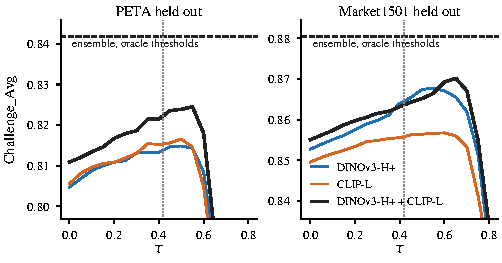
\includegraphics[width=\linewidth]{tau_rule.pdf}
\caption{Avg as a function of the coefficient $\tau$ on two held-out datasets. The dotted line marks our value and the dashed line the pair with oracle thresholds.}
\label{fig:tau}
\end{figure}

\subsection{Combining the encoders}
\label{sec:exp_design}

\Cref{tab:design} tests three alternatives to the equal-weight pair. The first changes the weights. On PETA the best weight is the equal weight. On Market1501 it moves towards DINOv3, which is as good alone as any mixture there. Equal weights stay within 0.11\pts{} of the best weight on both datasets, while using one encoder alone loses up to 0.91\pts. Equal weights are therefore a safe choice when the target domain is unknown.

The second alternative adds a third encoder. None of four candidates helps, including MetaCLIP2 ViT-H/14, the largest encoder we tried. A third encoder mostly repeats one that is already present, and its extra false positives cost as much as its corrections.

The third alternative replaces the pair with a single encoder of the same size. We distilled an ensemble of DINOv3 ViT-H+, CLIP ViT-L/14 and MetaCLIP2 ViT-H/14 into one DINOv3 ViT-H+ student~\cite{hinton}. The student alone is as accurate as the best single encoder. Paired with CLIP, however, it gains less than the original DINOv3, because it has copied CLIP's predictions and no longer disagrees with it. \Cref{fig:cases} shows why disagreement matters. For the backpack, DINOv3 is confident and right, CLIP is less confident and wrong, and the average follows DINOv3. The same figure shows the correction at work on a rare attribute, the pink top.

\begin{table}[t]
\centering\small
\setlength{\tabcolsep}{4pt}
\begin{tabular}{@{}lcc@{}}
\toprule
Variant & PETA & Market1501 \\
\midrule
Pair, equal weights (ours) & 82.33 & 86.35 \\
\quad weight of DINOv3 0.4 & 82.30 & 86.23 \\
\quad weight of DINOv3 0.6 & 82.29 & 86.46 \\
\midrule
+ MetaCLIP ViT-L/14 & 82.32 & -- \\
+ MetaCLIP2 ViT-H/14 & 82.27 & -- \\
+ AIMv2 ViT-L/14 & 82.16 & -- \\
+ SigLIP2 So400m/14 & 82.15 & -- \\
\midrule
distilled DINOv3 student alone & 82.00 & -- \\
distilled student + CLIP & 82.21 & -- \\
\bottomrule
\end{tabular}
\caption{Weighting the pair, adding a third encoder, and distilling the ensemble into one encoder.}
\label{tab:design}
\end{table}

\begin{figure*}[t]
\centering
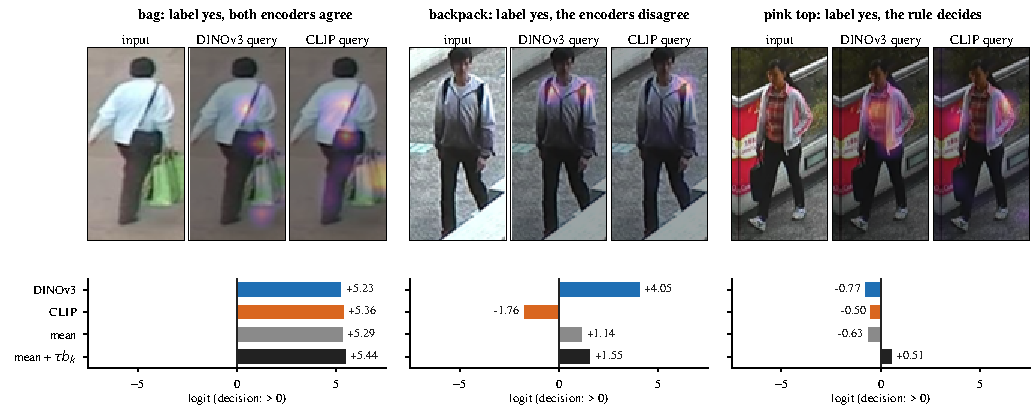
\includegraphics[width=\linewidth]{method_cases.pdf}
\caption{Three PETA cases for encoders that never saw PETA. Top: input and the attention of each encoder's query for the named attribute. Bottom: the logits of both encoders, their mean, and the mean after the prior correction.}
\label{fig:cases}
\end{figure*}

\subsection{How far to fine-tune}
\label{sec:exp_depth}

We also tried fine-tuning more deeply, with four frozen blocks and a decay of 0.9 instead of eight blocks and 0.75 (\cref{tab:depth}). This gives the middle blocks of ViT-H+ about twenty times larger learning rates. Deeper fine-tuning raises the source score of every encoder. On held-out data the effect is mixed. It helps DINOv3, hurts CLIP on PETA, and changes the pair only within the noise. On the hidden test set, the deeper pair scores 0.10\pts{} lower than the submitted one (\cref{sec:exp_test}). Fitting the training cameras more closely therefore does not pay off on new ones, and we keep the conservative setting.

\begin{table}[t]
\centering\small
\setlength{\tabcolsep}{3.2pt}
\resizebox{\columnwidth}{!}{%
\begin{tabular}{@{}lccc@{}}
\toprule
Model & source & PETA held out & Market1501 held out \\
\midrule
DINOv3 ViT-H+ & 88.66 $\rightarrow$ 89.17 & 81.42 $\rightarrow$ 82.01 & 86.46 $\rightarrow$ 86.64 \\
CLIP ViT-L & 88.38 $\rightarrow$ 88.82 & 81.54 $\rightarrow$ 81.10 & 85.60 $\rightarrow$ 85.63 \\
Pair (deeper DINOv3) & 89.14 $\rightarrow$ 89.35 & 82.33 $\rightarrow$ 82.51 & 86.35 $\rightarrow$ 86.42 \\
\bottomrule
\end{tabular}}
\caption{Conservative fine-tuning $\rightarrow$ deeper fine-tuning.}
\label{tab:depth}
\end{table}

\subsection{Hidden-test results}
\label{sec:exp_test}

\Cref{tab:test} lists our main submissions together with the held-out PETA score of the same recipe. The held-out score ranks the first three submissions in the same order as the test set. A single distilled DINOv3 ViT-L reaches 79.12. An ensemble of four models adds 0.63\pts. The DINOv3 ViT-H+ and CLIP ViT-L pair, which is smaller, adds another 0.22\pts{} and is our best submission. The held-out score of v20 uses a ten-epoch student instead of its longer-trained one. The deeper fine-tuning of \cref{sec:exp_depth} gains 0.18\pts{} on held-out PETA, inside the noise, and loses 0.10\pts{} on the test set. On the test set, our final system reaches an mA of 80.61 and an instance F1 of 79.33, with precision 75.61 and recall 84.90.

\begin{table}[t]
\centering\small
\setlength{\tabcolsep}{3pt}
\resizebox{\columnwidth}{!}{%
\begin{tabular}{@{}llcc@{}}
\toprule
& Models & PETA held out & Hidden test \\
\midrule
v13 & distilled DINOv3 ViT-L/16 & 81.18 & 79.12 \\
v20 & student + DINOv3 ViT-L + CLIP-L + MetaCLIP2-H & 82.03 & 79.75 \\
v21 & DINOv3 ViT-H+ + CLIP ViT-L (ours) & 82.33 & 79.97 \\
v22 & v21 with deeper fine-tuning & 82.51 & 79.87 \\
\bottomrule
\end{tabular}}
\caption{Our main submissions to UPAR 2027 Track~1.}
\label{tab:test}
\end{table}

%=====================================================================
\section{Conclusion}
\label{sec:conclusion}

We presented a system for pedestrian attribute recognition on unseen cameras with two components. Two foundation encoders with different pretraining, fine-tuned only in their upper blocks and averaged, improve ranking. A prior correction with one coefficient, derived from the metric, improves the decisions at the fixed threshold. Each component adds about one point on a held-out dataset, and the gains add up. Our experiments also give practical guidance. The partner encoder should be chosen by its held-out accuracy, equal weights are enough, and thresholds or fine-tuning tuned on the training data do not carry over to new cameras. The largest remaining error comes from labelling conventions of the target domain, which cannot be learned without some of its labels.

\paragraph{Limitations.}\label{sec:limits} Most comparisons use one held-out dataset and one run per setting, and the noise estimate comes from one encoder. \Cref{fig:arch,fig:cases} show ViT-L encoders of the same two families trained with the same settings, because the held-out version of the submitted ViT-H+ was not kept. The prior correction assumes that the training frequencies are estimated from representative data.

\paragraph{Broader impact.} Attribute recognition on surveillance video, including age and gender, can support the tracking of individuals. We report technical findings only and do not release models trained on surveillance data.

{\small
\bibliographystyle{ieeenat_fullname}
\bibliography{refs}
}

%=====================================================================
\clearpage
\appendix
\section{Training configuration}
\label{app:config}

Both encoders use the same settings. The optimizer is AdamW with a learning rate of $5\cdot10^{-5}$ at the last block, layer decay 0.75, a ten times larger learning rate for the head, weight decay 0.05 and batch size 64. The schedule is cosine with half an epoch of warm-up and lasts three epochs. Training uses stochastic depth 0.1, bf16 mixed precision and an exponential moving average of the weights with decay 0.9995, which is the model used at test time. The query head has one layer, eight attention heads, an MLP ratio of two and dropout 0.1. Augmentation consists of random down-scaling to simulate low resolution, horizontal flip, edge padding of ten pixels followed by a random crop, brightness, contrast and saturation jitter without hue change, Gaussian blur and random erasing. Attribute frequencies $\pi_k$ are clipped to $[10^{-3},1-10^{-3}]$, and labels that a dataset does not annotate are masked in the loss. At test time both encoders read the same crop resized to $224\times112$, and the pair processes the 29{,}248 test images in about four minutes on one NVIDIA A10 GPU.

\end{document}
